\documentclass{beamer}

\usepackage{préambule}
\usetikzlibrary{calc}

\newcommand\scalemath[2]{\scalebox{#1}{\mbox{\ensuremath{\displaystyle #2}}}}
\renewcommand{\vec}[1]{\scalemath{0.85}{\overrightarrow{#1}}}

\setbeamersize{
	text margin left=0.3cm,
	text margin right=0.3cm
}
\setlength{\leftmargini}{0.5cm}
\setlength{\leftmarginii}{0.3cm}

\begin{document}

\begin{frame}
	\footnotesize
	\begin{multicols}{2}
		\uline{Sujet A}
		\vspace*{-0.5cm}
		\begin{center}
			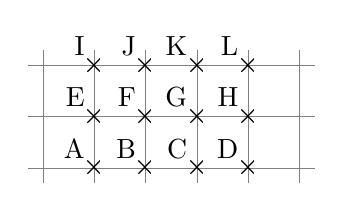
\begin{tikzpicture}[scale=0.65]
				\coordinate (A) at (0,0);
				\coordinate (B) at (1,0);
				\coordinate (C) at (2,0);
				\coordinate (D) at (3,0);
				\coordinate (E) at (0,1);
				\coordinate (F) at (1,1);
				\coordinate (G) at (2,1);
				\coordinate (H) at (3,1);
				\coordinate (I) at (0,2);
				\coordinate (J) at (1,2);
				\coordinate (K) at (2,2);
				\coordinate (L) at (3,2);
				\draw[very thin,gray] (-1.3,-0.3) grid (4.3,2.3);

				\foreach \p in {A,B,C,D,E,F,G,H,I,J,K,L} {
						\node at (\p) {×};
						\node[above left] at (\p) {\p};
					}
			\end{tikzpicture}
		\end{center}
		\begin{enumerate}
			\item \begin{enumerate}[a.]
				      \item Donner deux vecteurs égaux à $\vec{LD}$.
				      \item Donner un représentant de $\vec{AB} + \vec{BG}$.
				      \item Donner deux représentants de $\vec{EG} + \vec{HC}$.
				      \item Donner deux représentants de $\vec{KD} + \vec{FK} + \vec{CG}$.
			      \end{enumerate}
			\item Construire un triangle ABC rectangle en A, avec AB = 6cm et AC = 5cm.
			      \begin{enumerate}[a.]
				      \item Construire le point D tel que $\vec{AD} = \vec{CB}$.
				      \item Construire le point E tel que $\vec{BE} = \vec{AC} + \vec{AB}$.
			      \end{enumerate}
		\end{enumerate}

		\setlength{\columnseprule}{0.7pt}
		\columnbreak
		\setlength{\columnseprule}{0pt}

		\uline{Sujet B}
		\vspace*{-0.5cm}
		\begin{center}
			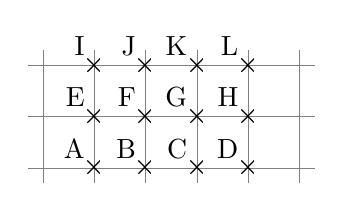
\begin{tikzpicture}[scale=0.65]
				\coordinate (A) at (0,0);
				\coordinate (B) at (1,0);
				\coordinate (C) at (2,0);
				\coordinate (D) at (3,0);
				\coordinate (E) at (0,1);
				\coordinate (F) at (1,1);
				\coordinate (G) at (2,1);
				\coordinate (H) at (3,1);
				\coordinate (I) at (0,2);
				\coordinate (J) at (1,2);
				\coordinate (K) at (2,2);
				\coordinate (L) at (3,2);
				\draw[very thin,gray] (-1.3,-0.3) grid (4.3,2.3);

				\foreach \p in {A,B,C,D,E,F,G,H,I,J,K,L} {
						\node at (\p) {×};
						\node[above left] at (\p) {\p};
					}
			\end{tikzpicture}
		\end{center}
		\begin{enumerate}
			\item \begin{enumerate}[a.]
				      \item Donner deux vecteurs égaux à $\vec{BJ}$.
				      \item Donner un représentant de $\vec{EF} + \vec{FG}$.
				      \item Donner deux représentants de $\vec{KF} + \vec{HG}$.
				      \item Donner deux représentants de $\vec{CA} + \vec{EB} + \vec{FG}$.
			      \end{enumerate}
			\item Construire un triangle ABC rectangle en A, avec AB = 5cm et AC = 6cm.
			      \begin{enumerate}[a.]
				      \item Construire le point D tel que $\vec{AD} = \vec{CB}$.
				      \item Construire le point E tel que $\vec{BE} = \vec{AC} + \vec{AB}$.
			      \end{enumerate}
		\end{enumerate}
	\end{multicols}
\end{frame}

\end{document}